\documentclass[border=6pt]{standalone}
\usepackage{amsmath}
\usepackage{tikz}
\usetikzlibrary{arrows.meta,calc,decorations.pathmorphing}
\begin{document}
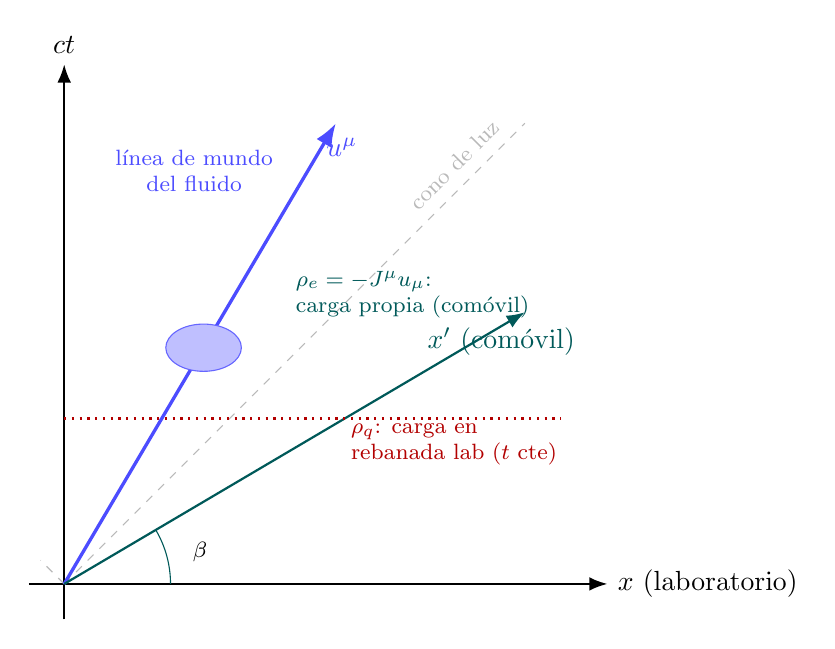
\begin{tikzpicture}[>=Latex,scale=1.5]

% ejes laboratorio (ct, x)
\draw[->,thick] (-0.3,0) -- (4.6,0) node[right] {$x$ (laboratorio)};
\draw[->,thick] (0,-0.3) -- (0,4.4) node[above] {$ct$};

% cono de luz
\draw[gray!55,dashed] (0,0) -- (3.9,3.9);
\draw[gray!55,dashed] (0,0) -- (-0.2,0.2);
\node[gray!55,font=\footnotesize,rotate=45] at (3.3,3.55) {cono de luz};

% linea de mundo del fluido = u^mu (timelike, pendiente >1)
\draw[->,very thick,blue!70] (0,0) -- (2.3,3.9);
\node[blue!70] at (2.35,3.7) {$u^\mu$};
\node[blue!70,font=\footnotesize,align=center] at (1.1,3.5) {línea de mundo\\ del fluido};

% eje espacial comovil x' (reflejo de u^mu respecto a 45°): pendiente = v = 0.59
\draw[->,thick,teal!70!black] (0,0) -- (3.9,2.3);
\node[teal!70!black] at (3.7,2.05) {$x'$ (comóvil)};

% elemento de fluido (blob) sobre la linea de mundo
\fill[blue!25,draw=blue!60] (1.18,2.0) ellipse (0.32 and 0.2);
\node[blue!60,font=\footnotesize] at (1.18,2.0) {};

% rho_q : medido en rebanada t=const del laboratorio (linea horizontal)
\draw[red!70!black,thick,dotted] (0,1.4) -- (4.2,1.4);
\node[red!70!black,font=\footnotesize,align=left] at (3.3,1.18)
  {$\rho_q$: carga en\\ rebanada lab ($t$ cte)};

% rho_e : medido en rebanada del marco comovil (paralela a x')
\draw[teal!60!black,thick,dotted] (0,0.0) ++(0,0) -- (0,0);
\node[teal!70!black,font=\footnotesize,align=left] at (2.95,2.45)
  {$\rho_e=-J^\mu u_\mu$:\\ carga propia (comóvil)};

% angulo entre x y x'
\draw[teal!70!black] (0.9,0) arc (0:30.5:0.9);
\node[font=\footnotesize] at (1.15,0.27) {$\beta$};

\end{tikzpicture}
\end{document}
